\documentclass{article}
\usepackage{graphicx}
\usepackage{algorithm}
\usepackage{algpseudocode} 

\usepackage[utf8]{inputenc}
\usepackage[english]{babel}
\setlength{\parindent}{0em}
\setlength{\parskip}{1em}


\usepackage{geometry}
 \geometry{
 a4paper,
 total={170mm,257mm},
 left=20mm,
 top=20mm,
 }
\usepackage{listings}

\usepackage{amsmath}
\DeclareMathOperator{\arcsec}{arcsec}

\begin{document}

\title{Laplace}

\author{2081052,2089602,2073835,2072566, 2091324}

\date{\today}

\maketitle

\begin{abstract}

\end{abstract}

\section{Introduction}

\begin{figure}[hp]
\centering
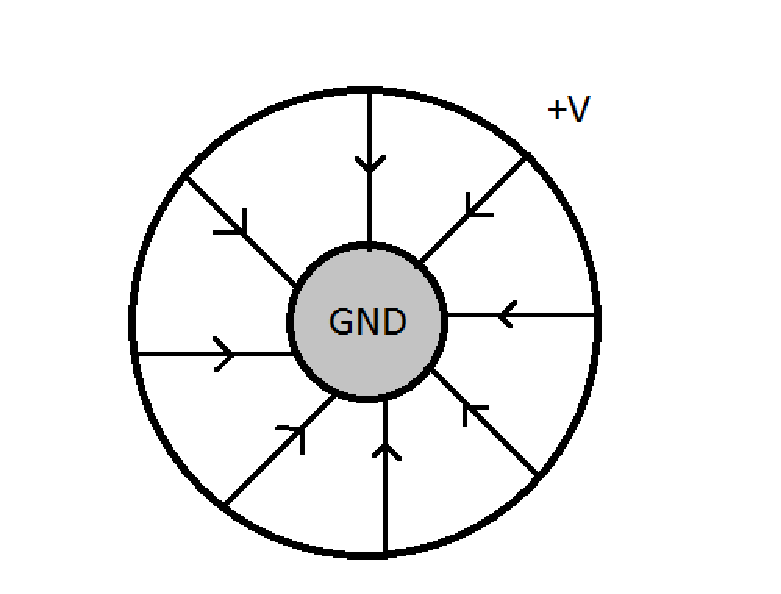
\includegraphics[width=75mm]{System1.pdf}
\caption{Diagram of system 1}
\label{fig:System1}
\end{figure}

\section{Analytical Solution}


 

\section{Numerical Solution}
\subsection{Methods}

It is not always possible to find an analytical solution as in real world 
situations the boundary conditions are not infinite. This means the systems
 need to be solved numerically and this is done using the finite difference
method.A relaxation method can be used to solve Poisson's equation.

The simplest method is the Jacobi's Iterative method. However, this method takes more iterations, i.e. more computing time, for the numerical answer to equal 
the analytical solution. 

\begin{equation} U_{n+1,j,k}=\frac{1}{4}\left [ U_{n,j+1,k} + U_{n,j-1,k} + U_{n,j,k+1} +U_{n,j,k-1}\right ]
\end{equation} 

Another method which is quicker is the Gauss-Seidel method. Unlike the Jacobi method it does not store the previous values and uses the points that have already been 'updated' to caluclate the next value.

\begin{equation}  
 U_{n+1,j,k}=\frac{1}{4}\left [ U_{n,j+1,k} + U_{n+1,j-1,k} + U_{n,j,k+1} +U_{n+1,j,k-1}\right ]
\end{equation}

The Successive Over Relaxation (SOR) method uses both the new and old solutions in a linear combination. 

\begin{equation}  
 U_{n+1,j,k}=\left (1-\omega)\right. U_{n,j,k}+\frac{\omega}{4}\left [ U_{n,j+1,k} + U_{n+1,j-1,k} + U_{n,j,k+1} +U_{n+1,j,k-1}\right ]
\end{equation}

The $\omega$ is the over-relaxation parameter and this can be changed to optimize the results. For a square lattice the SOR method converges fastest if: 

\begin{equation}
\omega \simeq \frac{2}{1 + \frac{\pi}{d}}
\end{equation}

where d is the number of grid points in either direction. \cite{numericalmethods}

\subsection{Method Comparison}

The different numerical methods were compared for System 2. The methods were compared for the following setup on the initial codes. Plates at voltage 10, distance 100, height 100, circle of radius 15 amd acceptable precision 0.001. 

The Jacobi method took 1514 iterations. This took a computing time of 0.94s.

The Gauss-Seidel method took 962 iterations. This took a computing time of 0.73s.

The SOR method took 165 iterations. This took a computing time of 0.28s.

It can clearly be seen that the best method is the SOR method. 

The following graph shows the rate of convergence of all three methods.

For the general solver the following setup was used to obtain the following results. Plates at voltage 5 and -5, distance and height 100, radius 10 and acceptable precision 0.001. 

The Jacobi method took 1113 iterations and 3.08s.

The Gauss-Seidel method took 822 iterations and 2.3s.

The SOR method took 496 iterations and 1.69s. 


\section{Structure of generic solver}

\section{Conclusion}


\section{Appendix}
\subsection{Algorithm of SOR method for System 2}
\begin{algorithm}
\begin{algorithmic}
\Procedure {The SOR method}{}
\State Initialise Variables
\State V - Potential on plates
\State d - Distance between plates
\State h - Height of plates
\State r- Radius of inner circle
\State error - Acceptable prescision
\State errorcount - Count error
\State omega =$ 2/(1+ \pi/d)$ - Relaxation parameter
\State dx, dy - Grid spacing
\State xstep = d/dx;
\State ystep = h/dy;
\State u[xstep +2][ystep +2] - Multidimensional array for potential
\State unew[xstep +2][ystep + 2] - Multidimensional array for updated potential
\State Boundary Conditions:
\For {int j=0; j$<$xstep; j++}
\For {int k=0; k$<$ystep;k++}
\If {j==0 $||$ j==xstep}
\State u[j][k]=V;
\State unew[j][k]=u[j][k];
\ElsIf{k==0 $||$ k==ystep}
\State u[j][k]=$V-(2*V*j)/xstep$;
\State unew[j][k]=u[j][k];
\Else
\State u[j][k]=0;
\State unew[j][k]=u[j][k];
\EndIf
\EndFor
\EndFor
\State SOR method:
\While {errorcount <xstep -1}
\State errorcount =0;
\For{int j=1;j$<$xstep;j++}
\For {int k=1;k$<$ystep;k++}
\If {Inside Ground Circle}
\State unew[j][k]=0;
\Else 
\State unew[j][k]=$(1-omega)*u[j][k]+(0.25)*(omega)*(unew[j-1][k]+u[j+1][k] + unew[j][k-1] + u[j][k+1]$;
\EndIf
\EndFor
\EndFor
\For {int j=0; j$<$xstep; j++}
\If {Convergence$<$error}
\State errorcount+=1;
\EndIf
\EndFor
\For {int j=1; j$<$(xstep); j++}
\For {int k=1;k$<$(ystep);k++}
\State u[j][k]=unew[j][k];
\EndFor
\EndFor
\EndWhile
\caption{SOR method Algorithm}
\EndProcedure
\end{algorithmic}
\end{algorithm}


\begin{thebibliography}{9}

\bibitem{numericalmethods}
Richard J. Gonsalves . 2011. \textit{Poisson's Equation and Relaxation Methods.} [ONLINE] Available at: http://www.physics.buffalo.edu/phy410-505/2011/topic3/app1/index.html. [Accessed 11 February 16]
	 
\end{thebibliography}
.

\end{document}
